% !TeX program = xelatex
% !BIB program = biber
\documentclass[12pt]{article}
\usepackage[margin=1in]{geometry}

% Fuente Times New Roman (compilar con XeLaTeX)
\usepackage{fontspec}
\setmainfont{Times New Roman}

% Idioma e interlineado
\usepackage[spanish,es-nodecimaldot]{babel}
\usepackage{setspace}
\setstretch{1.15}

% Paquetes principales
\usepackage{amsmath,amssymb}

% Marcado en azul de las correcciones incorporadas en la Entrega 2
\usepackage{xcolor}
\definecolor{azulcorr}{RGB}{0,0,205}
\newcommand{\corr}[1]{\textcolor{azulcorr}{#1}}
\newenvironment{correccion}{\par\color{azulcorr}}{\par}
\usepackage{tikz-cd}
\usepackage{multicol}
\usepackage{graphicx}
\usepackage{float}
\usepackage{booktabs}
\usepackage{caption}
\usepackage{titlesec}
\usepackage{enumitem}
\usepackage{longtable}
\usepackage{array}
\usepackage{xurl}
\usepackage{etoolbox}
\usepackage{placeins}

% Babel en espanol rotula las tablas como "Cuadro"; la prosa del documento las
% llama "Tabla" desde la Entrega 1.
\addto\captionsspanish{\renewcommand{\tablename}{Tabla}}

% Las paginas ocupadas solo por flotantes se alinean arriba y no al centro
\makeatletter
\setlength{\@fptop}{0pt}
\makeatother

% Figuras y tablas generadas por reports/Entrega 3.qmd
\graphicspath{{figuras/}}
\newcolumntype{P}[1]{>{\raggedright\arraybackslash}p{#1}}

\newcommand{\tabla}[1]{\input{tablas/#1}}

% Documento con muchas figuras: con los valores por defecto LaTeX se niega a
% poner un flotante en una pagina que ya tiene texto y deja huecos grandes.
\renewcommand{\topfraction}{0.9}
\renewcommand{\bottomfraction}{0.8}
\renewcommand{\textfraction}{0.07}
\renewcommand{\floatpagefraction}{0.75}
\setcounter{topnumber}{3}
\setcounter{totalnumber}{6}
% Sin flotantes al pie: tras una longtable el calculo de altura disponible de
% LaTeX se desajusta y un flotante inferior se desborda por debajo del margen.
\setcounter{bottomnumber}{0}
\usepackage{csquotes}
\usepackage[
  backend=biber,
  style=apa,
  sorting=nyt,
  sortcites=true
]{biblatex}
\DeclareLanguageMapping{spanish}{spanish-apa}
\addbibresource{referencias.bib}
% APA 7 en español: "Recuperado el [fecha], de [URL]".
\DefineBibliographyStrings{spanish}{retrieved = {Recuperado}, from = {de}}

% Formato APA 7 para la lista de referencias.
\setlength{\bibhang}{0.5in}
\AtBeginBibliography{\setstretch{1.15}}

% Compatibilidad con longtable de TeX Live 2025: evita diagnósticos espurios
% de contracción infinita al dividir tablas entre varias páginas.
\makeatletter
\patchcmd{\LT@output}{\copy\LT@foot\vss}{\copy\LT@foot\vfil}{}{}
\patchcmd{\LT@output}{\copy\LT@foot\vss}{\copy\LT@foot\vfil}{}{}
\makeatother

% Títulos, leyendas y numeración en 12 puntos
\titleformat{\section}
  {\normalfont\normalsize\bfseries}{\thesection}{1em}{}
\titleformat{\subsection}
  {\normalfont\normalsize\bfseries}{\thesubsection}{1em}{}
\titleformat{\subsubsection}
  {\normalfont\normalsize\bfseries}{\thesubsubsection}{1em}{}
\captionsetup{font=normalsize,labelfont=bf}
\titlespacing{\section}{0pt}{0pt}{0pt}
\titlespacing{\subsection}{0pt}{0pt}{0pt}
\captionsetup[figure]{belowskip=0pt}
\makeatletter
\patchcmd{\float@endH}{\box\@currbox\vskip\intextsep\relax}{\box\@currbox\relax}{}{\PackageError{figure-spacing}{No se pudo ajustar el espacio final de las figuras H}{Revise la definicion de float@endH.}}
\makeatother

% Párrafos
\setlength{\parindent}{1.5em}
\setlength{\parskip}{0pt}

% Numeración de páginas
\pagestyle{plain}

% Datos de la portada
\newcommand{\portadaUniversidad}{Universidad del Rosario}
\newcommand{\portadaPrograma}{Matemáticas Aplicadas y Ciencias de la Computación}
\newcommand{\portadaAsignatura}{Análisis Estadístico de Datos}
\newcommand{\portadaTitulo}{Factores socioeconómicos e institucionales asociados al desempeño en las pruebas Saber 11 (2020-2)}
\newcommand{\portadaIntegrantes}{%
  David Libreros\\
  Mateo Puente \\
  Nicolás González\\
  Santiago Díaz}
\newcommand{\portadaProfesora}{Luz Adriana Pineda Barón}
\newcommand{\portadaFecha}{\today}
\newcommand{\portadaSemestre}{Semestre 2026-2}

\begin{document}

% Portada
\begin{titlepage}
  \thispagestyle{empty}
  \centering

  {\bfseries \portadaUniversidad\par}
  \vspace{0.6cm}
  {\portadaPrograma\par}
  \vspace{0.4cm}
  {\portadaAsignatura\par}

  \vfill

  {\bfseries \portadaTitulo\par}

  \vfill

  {
    \textbf{Integrantes}\par
    \vspace{0.3cm}
    \portadaIntegrantes\par
    \vspace{0.8cm}
    \textbf{Profesora}\par
    \vspace{0.3cm}
    \portadaProfesora\par
  }

  \vfill

  {
    \portadaSemestre\par
    \portadaFecha\par
  }
\end{titlepage}

% La numeración visible comienza después de la portada.
\setcounter{page}{1}

\section{Introducción y planteamiento del problema}

El desempeño en las pruebas Saber 11 es un indicador de calidad educativa y un insumo para el
acceso a la educación superior en Colombia, y la literatura señala que no depende solo de factores
individuales, sino que está mediado por el contexto socioeconómico y familiar
\parencite{garciagil2021} y por las características del establecimiento y su ubicación
\parencite{quintero2025}. Este proyecto
analiza los resultados del segundo semestre de 2020, con información sociodemográfica, familiar,
institucional y de desempeño de unos 505.000 evaluados. El periodo corresponde a la primera
aplicación de la prueba en condiciones de pandemia, cuando las brechas de conectividad y de
acompañamiento familiar hicieron más notorias las diferencias entre contextos
\parencite{quintero2025}.

Aunque la prueba mide de manera estandarizada las competencias de todos los estudiantes al
finalizar el bachillerato, sus resultados no son homogéneos, pues quienes estudian en zonas
rurales o provienen de hogares con menor nivel socioeconómico muestran
patrones marcados de diferencia \parencite{morales2024}. Gran parte de los análisis se limita a
comparaciones descriptivas simples, de modo que queda un vacío sobre qué variables se asocian más
fuertemente con el desempeño y si esa asociación se mantiene al considerarlas de manera
simultánea.

\subsection{Pregunta de investigación}
¿En qué medida el conjunto de características individuales, familiares, socioeconómicas,
institucionales y geográficas registradas en la base de datos Saber 11 2020-2 se asocia con el
desempeño académico (puntaje global y por componente) de los estudiantes evaluados en Colombia?

\subsection{Objetivos}
El objetivo general es determinar el grado de asociación entre las características individuales,
familiares, institucionales y geográficas de los evaluados y sus colegios, y el desempeño obtenido
en Saber 11 2020-2, mediante técnicas de estadística multivariada. El primer objetivo específico
es caracterizar a la población evaluada según su género, edad, dedicación a la lectura y horas de
trabajo, y describir su relación con el desempeño. El segundo, analizar la asociación entre el
contexto familiar y socioeconómico y el desempeño. El tercero, explorar la relación entre las
características institucionales y geográficas del colegio y el desempeño de sus estudiantes. El
cuarto, identificar cuáles de esas variables presentan un mayor grado de asociación al examinarlas
de manera conjunta, medido mediante tamaños de efecto y varianza compartida, y en qué medida esa
asociación se superpone entre ellas.

\vspace{0.1cm}

\section{Revisión bibliográfica}

La literatura relaciona el rendimiento académico con el contexto individual, familiar y
socioeconómico. \textcite{garciagil2021} analizan la asociación entre las condiciones
socioeconómicas familiares y el desempeño en secundaria y bachillerato, \textcite{cruz2016}
construyen un índice socioeconómico para estudiantes de Saber 11 y \textcite{morales2024}
estudian la influencia del nivel socioeconómico familiar sobre el rendimiento. Para el periodo
cercano a la pandemia, \textcite{quintero2025} comparan los resultados de 2019-2 y 2021-2 y
encuentran una ampliación de las brechas entre colegios urbanos y rurales, y entre oficiales y
privados. Esta investigación amplía esos antecedentes mediante un enfoque
multivariado que las examina de manera conjunta en lugar de aislada.

\vspace{0.1cm}

\section{Marco metodológico y descripción de los datos}
\label{sec:metodologia}

\subsection{Fuente, población y variables}

Los datos provienen de la base pública Saber 11-2020-2 publicada por el ICFES en el portal de
Datos Abiertos del Gobierno Nacional de Colombia \parencite{icfes2026}, que reúne registros
administrativos de la inscripción y del examen con información sociodemográfica, del hogar, del
establecimiento educativo y los puntajes. El estudio es por tanto un análisis secundario de datos
oficiales públicos, procesado en \texttt{R} mediante Quarto para garantizar su reproducibilidad.
Como la prueba es obligatoria en grado 11 y reúne a todos los aspirantes sin selección previa, la
unidad de análisis es un censo de la población examinada y no una muestra probabilística, así que
la significancia estadística resulta poco informativa y la interpretación prioriza los tamaños de
efecto y la varianza explicada.

La base original contiene 504.872 observaciones y 81 variables. Primero se excluyeron los
identificadores y las variables constantes, redundantes o de pertinencia limitada, y después se
conservaron 12 de las 32 cualitativas restantes según su asociación con los puntajes ($\eta^2$) y
su redundancia con otras variables ($V$ de Cramér) y con el índice socioeconómico. El análisis trabaja así con 20 variables, 12 cualitativas y 8 cuantitativas,
descritas en la Tabla~\ref{tab:variables} de la Sección~\ref{anexo:variables}.

\subsection{Preparación de la base de datos}
\label{sec:preparacion}

No se hallaron registros duplicados. Se descartaron los 44 registros cuya validez está
condicionada a una actuación administrativa del ICFES, uno con cero en las cinco pruebas y 267
edades fuera del rango plausible de 13 a 100 años, el 0,05\,\% de la base original, mientras que los 257 con cero en
una prueba aislada se conservaron por tener puntajes válidos en las demás. Los faltantes se concentran en
las seis preguntas socioeconómicas, entre el 2,7 y el 3,4\,\%, y se clasificaron como pérdida
aleatoria condicional, o missing at random, pues la no respuesta se relaciona con menor puntaje
promedio (228,3 frente a 249,2) y mayor presencia en colegios oficiales y rurales, por lo que las
brechas estimadas probablemente están algo subestimadas. Se conservaron los registros completos
en esas preguntas, que tras los filtros suman 478.665 observaciones, base de todo el análisis. Las
variables categóricas se recodificaron como factores respetando el orden de las ordinales, dejando
\texttt{NO SABE}, \texttt{NO APLICA} y \texttt{SIN ESTRATO} fuera de la escala.

\vspace{0.1cm}

\section{Análisis descriptivo y exploratorio}
\label{sec:descriptivo}

\subsection{Variables cualitativas y cuantitativas}

El contexto socioeconómico de la población evaluada es de desventaja generalizada, pues el
90{,}0\,\% de los estudiantes pertenece a los estratos 1 a 3 y solo el 2{,}0\,\% a los estratos 5
y 6, el 30{,}0\,\% de los hogares carece de internet, limitación relevante ante el traslado de la
educación al hogar, y el 42{,}0\,\% tiene diez libros o menos. Predominan los colegios oficiales
(77{,}5\,\%) y urbanos (83{,}7\,\%), los niveles NSE 2 y NSE 3 del establecimiento concentran el
90{,}3\,\% y la educación materna se concentra en secundaria (41{,}9\,\%). El 58{,}2\,\% lee como
máximo media hora diaria y el 9{,}8\,\% trabaja más de veinte horas semanales, mientras que Bogotá
y Antioquia reúnen el 29{,}4\,\% de los evaluados.

\begin{figure}[H]
  \centering
  \begin{minipage}[c]{0.5\textwidth}
    \centering
    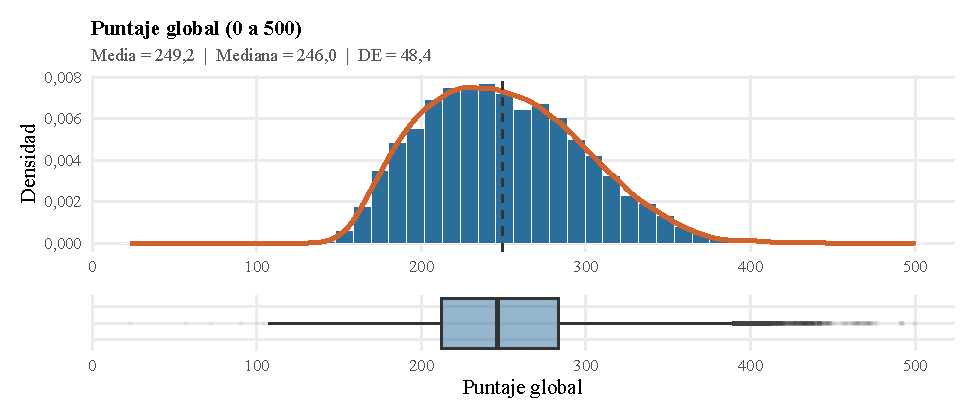
\includegraphics[width=\linewidth]{fig-global}
  \end{minipage}\hfill
  \begin{minipage}[c]{0.4\textwidth}
    \captionsetup{justification=raggedright,singlelinecheck=false,skip=0pt}
    \caption{Distribución del puntaje global en la escala de 0 a 500 puntos. Arriba el histograma
    con su curva de densidad y la media señalada por la línea discontinua, abajo la caja
    correspondiente sobre el mismo rango.}
    \label{fig:global}
  \end{minipage}
\end{figure}

La Figura~\ref{fig:global} muestra que el puntaje global es unimodal con leve asimetría positiva
(0{,}36), media de 249{,}2 puntos, mediana de 246{,}0 y desviación estándar de 48{,}4, con el
50\,\% central entre 212 y 283 puntos. En la escala común de 0 a 100 de los componentes, Lectura
Crítica presenta la mayor media (52{,}3) y la menor desviación (10{,}08), Sociales y Ciudadanas la
mayor desviación (11{,}93) e Inglés la menor media (47{,}1) junto con una cola de puntajes altos
(asimetría de 1{,}04). El índice socioeconómico es casi simétrico (media de 50{,}86 y desviación
de 9{,}46) y la edad muy asimétrica (8{,}26), por lo que su mediana de 17{,}4 años representa
mejor al estudiante típico.

\subsection{Relaciones bivariadas}
\label{sec:bivariado}

Se emplea el coeficiente $r$ de Pearson entre cuantitativas, cuyo cuadrado $r^2$ es la varianza
compartida. Entre una cualitativa y una cuantitativa se usa $\eta^2$, la proporción de la varianza
del puntaje debida a diferencias entre las medias de los grupos, y entre cualitativas, la $V$ de
Cramér. Ninguna implica causalidad.

\begin{figure}[H]
  \centering
  \begin{minipage}[c]{0.5\textwidth}
    \centering
    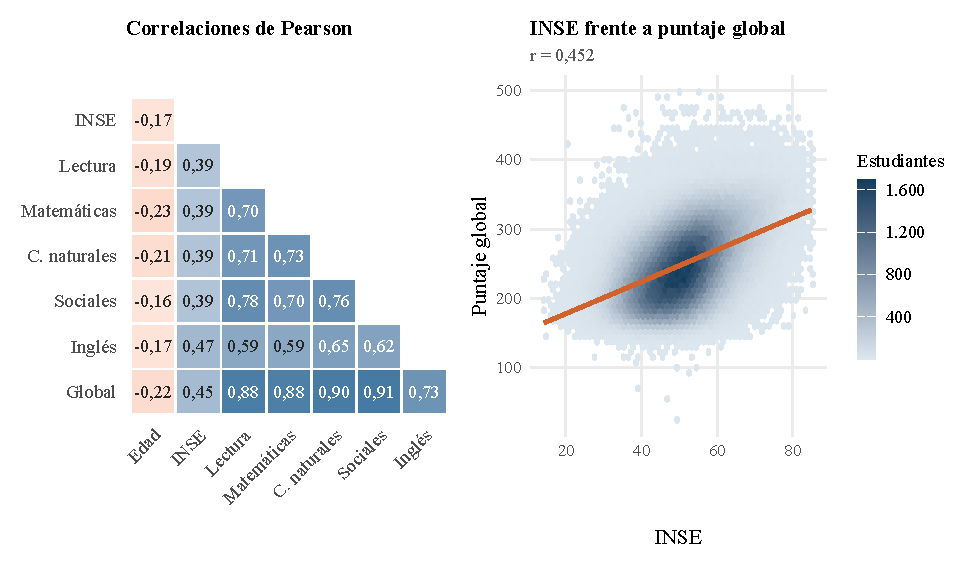
\includegraphics[width=\linewidth]{fig-corr-inse}
  \end{minipage}\hfill
  \begin{minipage}[c]{0.4\textwidth}
    \captionsetup{justification=raggedright,singlelinecheck=false,skip=0pt}
    \caption{Correlaciones de Pearson entre las ocho variables cuantitativas (izquierda) y
    relación entre el índice socioeconómico individual y el puntaje global (derecha). Los puntos
    se agrupan en hexágonos y el color codifica la densidad, porque con 478.665 observaciones una
    dispersión clásica produce una mancha uniforme.}
    \label{fig:corr-inse}
  \end{minipage}
\end{figure}

En la Figura~\ref{fig:corr-inse} los cinco componentes correlacionan entre 0{,}59 y 0{,}78, más
entre Lectura Crítica y Sociales y menos con Inglés, lo que respalda su análisis conjunto. El
índice socioeconómico se asocia moderadamente con el puntaje global ($r = 0{,}452$) y más con
Inglés (0{,}47) que con las demás pruebas (0{,}39), y la edad lo hace de forma débil y negativa
($r = -0{,}22$). La nube de hexágonos crece de manera sostenida y sin tramos planos, de modo que
la relación es aproximadamente lineal en todo el rango del índice.

\begin{figure}[H]
  \centering
  \begin{minipage}[c]{0.5\textwidth}
    \centering
    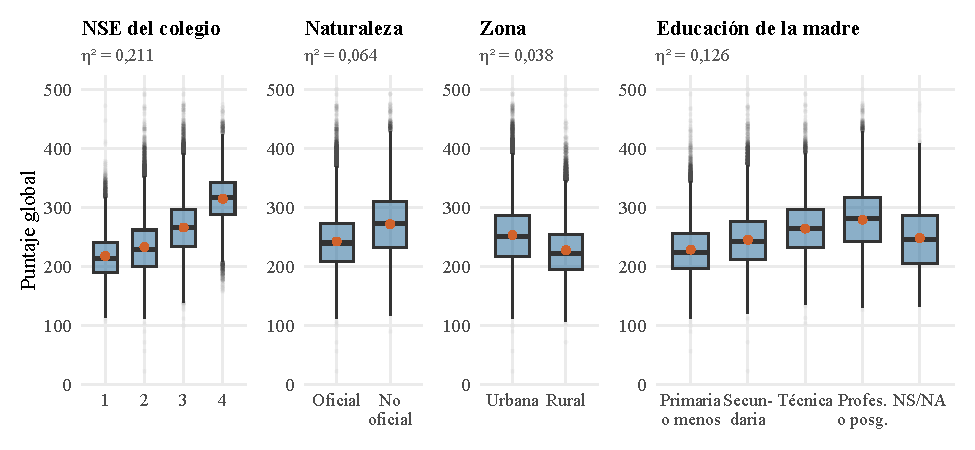
\includegraphics[width=\linewidth]{fig-box-clave}
  \end{minipage}\hfill
  \begin{minipage}[c]{0.4\textwidth}
    \captionsetup{justification=raggedright,singlelinecheck=false,skip=0pt}
    \caption{Puntaje global según el nivel socioeconómico, la naturaleza y la zona del colegio y la
    educación de la madre. El punto naranja marca la media de cada grupo. El $\eta^2$ de la
    educación materna se calcula aquí sobre la variable agrupada en cuatro niveles más
    No sabe o No aplica, por lo que difiere del de la Tabla~\ref{tab:asociacion}.}
    \label{fig:box-clave}
  \end{minipage}
\end{figure}

La Figura~\ref{fig:box-clave} muestra brechas relevantes frente a una desviación estándar global
de 48{,}4 puntos. Los colegios no oficiales promedian 271{,}9 puntos frente a 242{,}6 de los
oficiales y los urbanos 253{,}3 frente a 228{,}0 de los rurales, mientras que el promedio aumenta
de 217{,}9 en NSE 1 a 314{,}8 en NSE 4 y de 228{,}8 a 279{,}3 entre madres con primaria o menos y
madres con estudios profesionales. La Tabla~\ref{tab:asociacion} confirma que las mayores
asociaciones con el puntaje global son las del NSE del colegio (21{,}1\,\%), el índice
socioeconómico individual (20{,}4\,\%) y la educación materna (14{,}2\,\%), frente a la
naturaleza del colegio (6{,}4\,\%), la lectura (2{,}5\,\%) o el género (0{,}5\,\%). Inglés es el
componente más sensible al contexto, pues el NSE del colegio alcanza allí el 24{,}4\,\% y la
naturaleza el 9{,}4\,\%, frente a valores entre 4{,}3 y 5{,}1\,\% de esta última en las demás
pruebas, mientras que el género llega a su máximo en Matemáticas (1{,}6\,\%). El puntaje global
oculta entonces diferencias entre áreas, lo que justifica analizar cada componente.

\tabla{tab-asociacion}

Entre las cualitativas, las asociaciones más fuertes se concentran también en el bloque
socioeconómico e institucional. El NSE del colegio se asocia con su naturaleza ($V = 0{,}54$), su
zona (0{,}48) y el acceso a internet del hogar (0{,}46), la naturaleza con la jornada (0{,}53) y
el estrato con el acceso a internet (0{,}38), mientras que el género, la lectura y el trabajo no
superan $V = 0{,}20$ con ninguna otra. El par más asociado ilustra la segregación del sistema, ya
que el 20{,}9\,\% de los estudiantes de colegios no oficiales está en NSE 4, nivel casi
inexistente entre los oficiales, donde el 61{,}9\,\% está en NSE 2. Estas superposiciones definen
la agenda del análisis multivariado, que consiste en cuantificar el aporte propio de cada
dimensión y examinar la estructura conjunta del desempeño y del contexto.

\vspace{0.1cm}

\section{Metodología estadística}
\label{sec:met-estadistica}

\subsection{Técnicas seleccionadas y justificación}

La elección de las técnicas parte de tres rasgos del problema. La respuesta no es una variable
sino un vector de cinco puntajes continuos que correlacionan entre 0,59 y 0,78, y el puntaje
global no puede acompañarlos por ser un promedio ponderado de ellos. Las doce explicativas del
modelo son cualitativas, pues la edad entra por tramos, y el índice socioeconómico individual, el
único predictor continuo, solo interviene en la especificación alternativa. Y el diseño es
observacional sobre la población completa, de modo que el objetivo es cuantificar
asociaciones y no efectos causales. Quedan así fuera la clasificación supervisada,
porque no hay una variable de grupo que predecir, y el agrupamiento, porque el interés no está en
segmentar estudiantes sino en medir relaciones entre bloques definidos de antemano.

Las dos primeras técnicas resumen conjuntos de variables. El análisis de componentes principales
se aplica a los cinco puntajes sobre la matriz de correlaciones, para que las diferencias de
dispersión entre pruebas no determinen la solución, y se valida con la medida de adecuación de
Kaiser-Meyer-Olkin y la prueba de esfericidad de Bartlett \parencite{johnson2007}. El de
correspondencias múltiples cumple la función equivalente sobre las nueve variables cualitativas
del contexto, que el anterior no puede tratar, proyectando sus categorías a partir de la tabla
disyuntiva \parencite{greenacre2017}. Las características individuales y los puntajes entran allí
como suplementarios, sin participar en la construcción de los ejes. Ambas son descriptivas y no
establecen dependencia. La segunda añade dos cautelas, pues sus inercias brutas subestiman la
varianza explicada y exigen las correcciones de Benzécri y Greenacre, y su segundo eje tiende a
reproducir el primero en forma de herradura, artefacto conocido como efecto Guttman.

La regresión lineal multivariada responde la pregunta de dependencia. Las cinco respuestas
comparten predictores, así que se estiman en un solo modelo cuyos coeficientes coinciden con los
de cinco regresiones separadas pero que permite contrastar hipótesis sobre todas a la vez
\parencite{diaz2012}. Las doce explicativas se agrupan en cuatro bloques, que son las
características individuales, el hogar, el establecimiento y la geografía, y el aporte propio de
cada uno se mide como la caída del $R^2$ al retirarlo, mientras que su diferencia con la
asociación aislada mide la superposición. El contraste conjunto usa el estadístico de Pillai, el
más robusto ante desviaciones de la normalidad multivariada, aunque con una base de este tamaño
cualquier diferencia resulta significativa y la lectura se apoya en la varianza explicada. El
modelo supone efectos aditivos, y el contexto socioeconómico se representa de dos maneras
alternativas, las preguntas crudas del hogar y los índices del ICFES, cuyos $R^2$ se comparan.

\subsection{Preparación adicional de las variables}

Las técnicas factoriales son sensibles a las categorías poco frecuentes, que reciben coordenadas
extremas y distorsionan los ejes, así que varias se agruparon. Los 32 departamentos pasaron a
seis regiones, con Bogotá separada por su tamaño y su perfil propio, los once niveles de educación
materna a cinco y los estratos 5 y 6 a uno solo, con un costo bajo, pues el $\eta^2$ con el
puntaje global baja de 6,8 a 4,6\,\% en la geografía y de 14,2 a 12,6\,\% en la educación
materna. La edad pasó a cinco tramos por otra razón, ya que su relación con el puntaje no es
lineal y el $\eta^2$ por tramos, del 9,4\,\%, duplica el $r^2$ de la versión continua. Los factores
ordinales se reexpresaron con contrastes de tratamiento, que no alteran el $R^2$ y permiten leer
cada categoría frente a una de referencia.

\vspace{0.1cm}

\section{Verificación de supuestos}
\label{sec:supuestos}

Los supuestos se verificaron para cada técnica con sus propias variables: la adecuación muestral del
ACP, con los cinco puntajes, y los supuestos de la regresión, con las doce
variables explicativas del modelo. Con una muestra de este tamaño las pruebas
formales rechazan cualquier desviación, por lo que se evalúan magnitudes (KMO, VIF, momentos de los
residuos) y no valores $p$ (Tabla~\ref{tab:supuestos}).

\begin{table}[H]
  \centering
  \caption{Verificación de los supuestos de la regresión y del ACP.}
  \label{tab:supuestos}
  \footnotesize\setstretch{1}\setlength{\tabcolsep}{4pt}
  \begin{tabular}{P{4.8cm} P{7.4cm} P{2.8cm}}
    \toprule
    \textbf{Supuesto y qué exige} & \textbf{Evidencia (criterio)} & \textbf{Veredicto} \\
    \midrule
    \textbf{Correlación entre los puntajes (ACP)}: los puntajes comparten información suficiente
    para resumirse en pocos componentes & KMO de 0{,}885, con 0{,}858 a 0{,}936 por variable (criterio: mayor que 0{,}5);
    Bartlett significativo, aunque poco informativo con este $n$ & \textbf{Cumple} \\
    \textbf{Multicolinealidad}: las explicativas no son redundantes entre sí & GVIF$^{1/\mathrm{gl}}$,
    equivalente al VIF para predictores con varios grados de libertad, entre 1{,}02 y 1{,}68, con
    máximo de 4{,}48 al añadir los índices del ICFES (criterio: menor que 5) &
    \textbf{Cumple} \\
    \textbf{Normalidad}: los residuos tienen forma de campana & Asimetría de 0{,}03 a 0{,}18 y
    curtosis de 0{,}15 a 0{,}62; en Inglés, 0{,}62 y 1{,}31 (criterio: valores cercanos a 0) &
    \textbf{Cumple}, con desviación leve en Inglés (cola derecha) \\
    \textbf{Homocedasticidad}: el error tiene dispersión constante & Desviación estándar de los
    residuos por decil del valor ajustado entre 8{,}11 y 8{,}98 (criterio: dispersión similar) &
    \textbf{Cumple} \\
    \textbf{Linealidad} (INSE): cada punto de INSE suma un puntaje constante & $r^2 = 0{,}204$ frente a
    $\eta^2 = 0{,}203$ de los deciles (criterio: valores casi iguales) & \textbf{Cumple} \\
    \textbf{Independencia}: los errores de distintos estudiantes no se relacionan & Estudiantes
    anidados en colegios, estructura que el modelo no incorpora. El identificador del
    establecimiento existe en la base publicada, pero se excluyó al seleccionar variables &
    \textbf{No cumple}: errores estándar subestimados, $R^2$ y tamaños de efecto intactos \\
    \bottomrule
  \end{tabular}
\end{table}

El ACM no estima un modelo de dependencia y solo exige frecuencias suficientes por categoría, lo que
garantiza la agrupación de la Sección~\ref{sec:met-estadistica}. En conjunto, los supuestos se cumplen
salvo la independencia y una leve desviación de la normalidad en Inglés, sin que esto invalide una
lectura basada en tamaños de efecto.

\vspace{0.1cm}

\section{Aplicación de la metodología}
\label{sec:aplicacion}

\subsection{Estructura del desempeño}

El análisis de componentes principales, con los 478.445 registros que tienen los cinco puntajes
completos, encuentra una estructura marcadamente unidimensional. La
primera componente recoge el 74,7\,\% de la varianza y la segunda el 9,2\,\%, y las cinco pruebas
cargan positivamente y con intensidad parecida sobre el primer eje, entre 0,790 en Inglés y 0,897
en Sociales y Ciudadanas, lo que identifica un factor general de desempeño. La segunda separa a Inglés
del resto, con una correlación de 0,605 frente a valores entre $-0{,}221$ y $-0{,}028$ en los
otros cuatro, de modo que es un eje de especificidad en lengua extranjera. Eso justifica modelar
los cinco puntajes y no solo el global, porque un resumen único borraría esa diferencia.

\subsection{Estructura del contexto}

El análisis de correspondencias múltiples se calculó con nueve variables activas que aportan 37
categorías y generan 28 dimensiones, sobre los 478.171 registros completos también en las
suplementarias. Las inercias brutas reparten la variación entre muchos ejes, de modo que el
primer eje recoge en bruto apenas el
11,7\,\% del total, pero una vez corregido el sesgo de la codificación disyuntiva concentra el
73,6\,\% de la inercia según Greenacre, o el 83,5\,\% con Benzécri.

\begin{figure}[H]
  \centering
  \begin{minipage}[c]{0.5\textwidth}
    \centering
    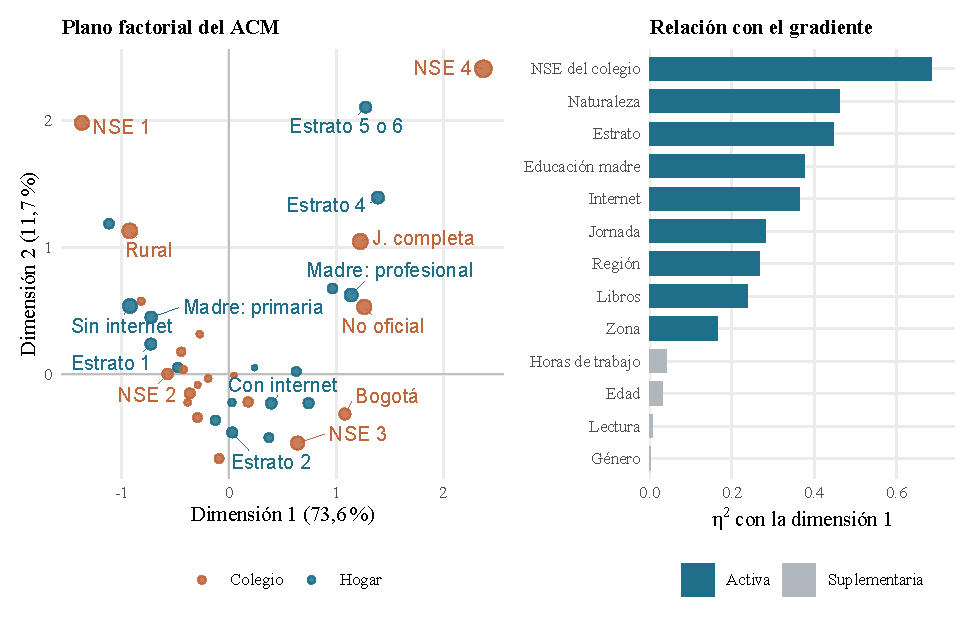
\includegraphics[width=\linewidth]{fig-acm-plano}
  \end{minipage}\hfill
  \begin{minipage}[c]{0.4\textwidth}
    \captionsetup{justification=raggedright,singlelinecheck=false,skip=0pt}
    \caption{Primer plano factorial del análisis de correspondencias, con el tamaño del punto
    proporcional a la contribución de la categoría y rótulos en las dieciséis más influyentes
    (izquierda), y $\eta^2$ de cada variable con la primera dimensión, distinguiendo las activas
    de las suplementarias (derecha). Los porcentajes de inercia son los corregidos por
    Greenacre.}
    \label{fig:acm-plano}
  \end{minipage}
\end{figure}

La Figura~\ref{fig:acm-plano} muestra que ese gradiente ordena las categorías de menor a mayor
ventaja socioeconómica, con los colegios no oficiales y las madres con estudios profesionales en
el extremo positivo, y la ausencia de internet, el estrato 1 y la zona rural en el negativo. Las variables del hogar y las del colegio se mezclan a lo largo del
eje en lugar de ocupar zonas separadas, lo que indica que la ventaja familiar y la institucional
son caras de una misma condición. Las más relacionadas con el eje son el nivel
socioeconómico del colegio, con $\eta^2 = 0{,}686$, la naturaleza con 0,460 y el estrato con 0,448.

El contraste con las variables suplementarias es el resultado más informativo de este análisis.
Ninguna característica individual alcanza un $\eta^2$ de 0,05 con el primer eje, de modo que el
bloque individual es casi ortogonal al gradiente socioeconómico y constituye una fuente de
variación distinta. Los cinco puntajes se proyectan sobre el eje con coordenadas de entre 0,415 y
0,426, salvo Inglés que llega a 0,508. La segunda dimensión no aporta variación nueva, pues sus
mayores contribuciones provienen de los dos extremos del gradiente situados del mismo lado del
eje, el efecto Guttman anticipado en la Sección~\ref{sec:met-estadistica}.

\subsection{Modelo de dependencia}

El modelo lineal multivariado explica entre el 25,0 y el 29,6\,\% de la varianza de cada
componente, con el máximo en Inglés y el mínimo en Lectura Crítica. Tomado de forma aislada, el
contexto del hogar es el bloque más asociado en los cinco casos, con valores entre 15,4 y
21,8\,\%, seguido del establecimiento con 12,4 a 16,7\,\%, las características individuales con
10,6 a 13,5\,\% y la geografía con 3,3 a 3,8\,\%. El estadístico de Pillai rechaza la nula para
los doce predictores, resultado esperable y poco informativo aquí.

\tabla{tab-aportes}

El orden cambia al descontar lo que cada bloque comparte con los demás. La
Figura~\ref{fig:aportes} muestra que el aporte propio del hogar cae a entre 3,9 y 6,7 puntos de
varianza y el del establecimiento a entre 2,0 y 2,8, mientras que el bloque individual conserva
entre 2,9 y 5,2 pese a partir de una asociación aislada menor. El mismo fenómeno aparece variable
por variable en la Tabla~\ref{tab:aportes}, donde la educación de la madre pasa del 12,6\,\%
aislado al 1,7\,\% propio. Sobre el puntaje global, las doce variables explican en conjunto el
33,0\,\% frente a un 80,2\,\% sumando sus asociaciones por separado.

\begin{figure}[H]
  \centering
  \begin{minipage}[c]{0.5\textwidth}
    \centering
    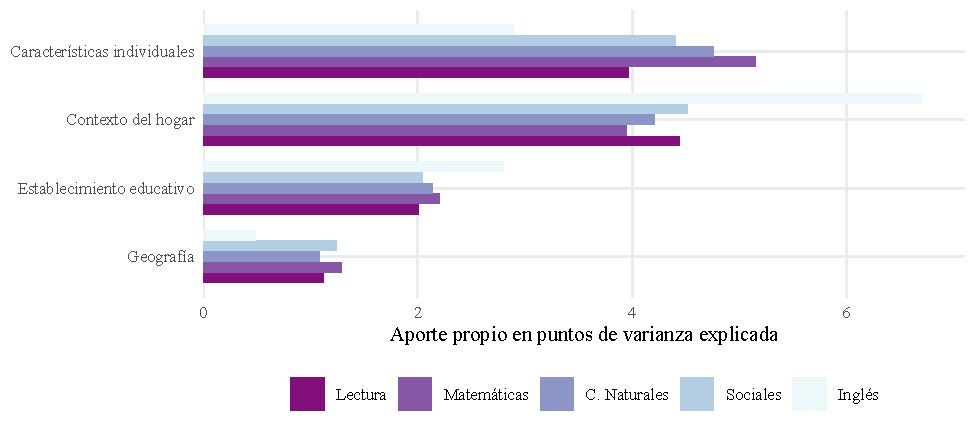
\includegraphics[width=\linewidth]{fig-aportes}
  \end{minipage}\hfill
  \begin{minipage}[c]{0.4\textwidth}
    \captionsetup{justification=raggedright,singlelinecheck=false,skip=0pt}
    \caption{Aporte propio de cada bloque a la varianza explicada de cada componente, medido como
    la caída del $R^2$ del modelo completo al retirar el bloque. Las asociaciones aisladas son
    bastante mayores, y la diferencia corresponde a la varianza que los bloques comparten entre
    sí.}
    \label{fig:aportes}
  \end{minipage}
\end{figure}

Esa superposición no se manifiesta como colinealidad entre predictores, sino como la porción de
varianza del puntaje que cada variable comparte con las demás, visible solo al descomponer el
$R^2$. El género ilustra el caso contrario, ya que su asociación aislada es del 0,52\,\% y su
aporte propio del 0,91\,\%, una parte compartida negativa que indica supresión. El mecanismo está
en su relación con las demás explicativas, pues los hombres trabajan más horas y leen menos,
rasgos asociados a puntajes bajos que enmascaran parte de su ventaja, de modo que la brecha sube
de 7,0 a 9,6 puntos al controlar el resto del modelo. La comparación entre las dos representaciones del nivel socioeconómico
favorece a los índices del ICFES, pues sustituir las cuatro preguntas crudas del hogar por el
índice individual y el nivel del establecimiento eleva el $R^2$ de los cinco componentes, de 29,6
a 33,4\,\% en Inglés.

\vspace{0.1cm}

\section{Discusión de resultados}
\label{sec:discusion}

Los resultados coinciden con la literatura en la dirección de las asociaciones. La relación entre
condiciones socioeconómicas familiares y rendimiento que reportan \textcite{garciagil2021} y
\textcite{morales2024} se refleja en el 20,4\,\% de varianza del puntaje global asociado al índice
socioeconómico individual y en brechas de 0,61 y 0,52 desviaciones estándar entre naturalezas y
zonas de colegio, aunque una brecha entre grupos muy desbalanceados puede explicar poca varianza,
como el 3,8\,\% de la zona.

El principal aporte es cuantificar la redundancia. Examinar los factores por separado, como hacen
los estudios citados, sobrestima su peso independiente por un factor cercano a seis, pues las
asociaciones aisladas suman el 80,2\,\% de la varianza del puntaje global frente al 13,5\,\% que
suman los aportes propios. También altera el orden, pues la educación de la madre pasa de
encabezar las asociaciones aisladas a una posición modesta. La causa es que hogar y colegio colapsan en un único gradiente en el ACM y, con la
segregación escolar ($V = 0{,}54$ entre naturaleza y NSE del establecimiento), las variables de uno
transportan buena parte de la información del otro.

El estudio respalda el índice de \textcite{cruz2016}, propuesto por razones conceptuales y de
medición, ya que sustituirlo por las preguntas crudas del hogar reduce el $R^2$ de los cinco
componentes. Confirma también las brechas urbano-rural y oficial-privada de \textcite{quintero2025},
sin poder evaluar su ampliación entre 2019-2 y 2021-2 por ser un único corte, y muestra que no son
independientes entre sí ni del hogar, por lo que no conviene leerlas como efectos separados del
sistema escolar.

Dos hallazgos carecen de antecedente directo. Las características individuales, de asociación
débil, son casi ortogonales al gradiente socioeconómico y aportan variación propia. Inglés se aísla
en el segundo eje del ACP y tiene el mayor $R^2$ y la mayor proyección sobre el gradiente, lo que
sugiere mayor dependencia de la exposición fuera de la escuela. Todo lo anterior describe
asociaciones, no efectos causales.

\vspace{0.1cm}

\section{Conclusiones}
\label{sec:conclusiones}

\begin{enumerate}[leftmargin=*,itemsep=2pt,topsep=2pt]
  \item Las características individuales, familiares, institucionales y geográficas se asocian de forma relevante pero parcial con el desempeño, pues explican entre el 25,0 y el 29,6\,\% de la varianza de cada componente y el 33,0\,\% del puntaje global, dejando sin explicar cerca de dos tercios de este último.

  \item Respecto al segundo y tercer objetivo, el contexto socioeconómico es el factor más asociado. El NSE del colegio (21,1\,\%) y el índice individual (20,4\,\%) encabezan las asociaciones con el puntaje global, y el hogar (15,4 a 21,8\,\%) y el establecimiento (12,4 a 16,7\,\%) son los bloques más asociados en los cinco componentes, en línea con las brechas entre colegios no oficiales y oficiales (271,9 frente a 242,6 puntos) y entre urbanos y rurales (253,3 frente a 228,0).

  \item Respecto al cuarto objetivo, la conclusión central es que ese peso no es independiente. Hogar y colegio forman un gradiente único que concentra el 73,6\,\% de la inercia del ACM, por lo que las asociaciones aisladas suman el 80,2\,\% frente al 33,0\,\% conjunto, y al descontar lo compartido el aporte propio del hogar cae a entre 3,9 y 6,7 puntos y el del establecimiento a entre 2,0 y 2,8. No pueden leerse como efectos separados.

  \item Respecto al primer objetivo, las características individuales (edad, trabajo, lectura y género) pesan menos que el contexto, pero conservan un aporte propio de 2,9 a 5,2 puntos y, al ser casi ortogonales al gradiente, son una fuente de variación distinta.

  \item Un factor general recoge el 74,7\,\% de la varianza de los puntajes, pero Inglés se separa en un segundo eje y tiene la mayor varianza explicada (29,6\,\%), lo que justifica analizar cada prueba y no solo el puntaje global.
\end{enumerate}

\vspace{0.1cm}

\section{Limitaciones del estudio}
\label{sec:limitaciones}

\begin{enumerate}[leftmargin=*,itemsep=2pt,topsep=2pt]
  \item El diseño observacional y de un único corte (2020-2) solo permite describir asociaciones, no efectos causales ni la evolución de las brechas.

  \item El modelo explica el 33{,}0\,\% de la varianza del puntaje global, y cerca de dos tercios responden a factores no registrados, como el desempeño previo o la calidad de la enseñanza.

  \item Los estudiantes están anidados en colegios y el modelo no incorpora esa estructura, lo que viola la independencia y subestima los errores estándar, sin afectar los $R^2$ ni los tamaños de efecto. El identificador del establecimiento existe en la base publicada, así que la limitación es del alcance del análisis y no de los datos.

  \item La no respuesta socioeconómica no fue completamente aleatoria, por lo que las brechas probablemente están algo subestimadas. La agrupación de categorías para las técnicas factoriales restó algo de detalle (el $\eta^2$ de la geografía bajó de 6{,}8 a 4{,}6\,\%), y el modelo supone efectos aditivos entre bloques.
\end{enumerate}

\vspace{0.1cm}

\section{Recomendaciones}
\label{sec:recomendaciones}

Estas recomendaciones se derivan de las limitaciones anteriores:

\begin{enumerate}[leftmargin=*,itemsep=2pt,topsep=2pt]
  \item Frente a la falta de independencia, la misma base permite recuperar el identificador del establecimiento (\texttt{COLE\_CODIGO\_ICFES}) para agrupar los errores estándar por colegio o ajustar un modelo multinivel, que separaría la variación entre colegios de la existente dentro de cada uno y respondería cuánto del gradiente socioeconómico corresponde al hogar y cuánto al entorno escolar.
  
  \item Para superar el corte transversal, se podría replicar el análisis con otras aplicaciones de Saber 11, como 2019-2 y 2021-2, y comprobar si el gradiente y su redundancia se mantienen en el tiempo, incorporando variables hoy ausentes como el desempeño previo.
  
  \item Frente a la no respuesta, la imputación múltiple permitiría contrastar los resultados con los de casos completos y medir cuánto se subestiman las brechas.
  
  \item Incluir interacciones entre bloques, por ejemplo entre naturaleza y zona del colegio, permitiría evaluar el supuesto de aditividad.
\end{enumerate}

\newpage

\section{Declaración de uso de inteligencia artificial}
Se usaron herramientas de Inteligencia Artificial (IA) para el desarrollo de esta entrega, para fines como mejorar la redacción, 
depurar código, automatizar cosas como exportar tablas y figuras a \LaTeX, manejo de pipelines, definir estilos para mantener consistencia,
documentación sobre el uso de herramientas como Quarto y R, replantear enfoques o decisiones posiblemente erróneas y revisar
el documento contra la guía de la entrega para verificar que cumpliera sus requisitos.
En general se buscó con estas herramientas elevar la calidad del trabajo. La interpretación de los
resultados, las conclusiones y las decisiones metodológicas fueron realizadas por el grupo.

Entre las herramientas utilizadas se encuentran:
\begin{itemize}
  \item Claude (Opus 5)
  \item OpenAI Prism
\end{itemize}

\vspace{0.1cm}

\section{Participación del grupo}

Santiago Díaz realizó el planteamiento de los modelos, su ejecución y el análisis, Mateo Puente
el póster y la parte introductoria del documento, David Libreros la verificación de supuestos y
las conclusiones, y Nicolás González las limitaciones y las recomendaciones.

\vspace{0.1cm}

\section{Variables seleccionadas}
\label{anexo:variables}

\begingroup\small\setlength{\tabcolsep}{4pt}
\newcolumntype{L}[1]{>{\raggedright\arraybackslash}p{#1}}
\begin{longtable}{L{5.8cm} L{2.0cm} L{1.6cm} L{5.8cm}}
  \caption{Descripción de las variables seleccionadas para el análisis.}\label{tab:variables}\\
  \toprule
  \textbf{Variable} & \textbf{Tipo} & \textbf{Escala} & \textbf{Descripción} \\
  \midrule
  \endfirsthead

  \midrule
  \multicolumn{4}{r}{\textit{Continúa en la página siguiente...}} \\
  \midrule
  \textbf{Variable} & \textbf{Tipo} & \textbf{Escala} & \textbf{Descripción} \\
  \midrule
  \endhead

  \midrule
  \multicolumn{4}{r}{\textit{Continúa en la página siguiente...}} \\
  \endfoot

  \bottomrule
  \endlastfoot

  \midrule
  \multicolumn{4}{l}{\textit{Características demográficas}} \\
  \texttt{ESTU\_GENERO} & Cualitativa & Nominal & Género reportado por el estudiante. \\
  \texttt{ESTU\_FECHANACIMIENTO} & Cuantitativa & Intervalo & Fecha de nacimiento; se usa solo para calcular la edad. \\
  \texttt{EDAD} & Cuantitativa & Razón & Variable derivada: edad al 7 de noviembre de 2020, primera fecha de aplicación \\

  \midrule
  \multicolumn{4}{l}{\textit{Hábitos y dedicación}} \\
  \texttt{ESTU\_DEDICACIONLECTURADIARIA} & Cualitativa & Ordinal & Tiempo diario dedicado a la lectura por entretenimiento. \\
  \texttt{ESTU\_HORASSEMANATRABAJA} & Cualitativa & Ordinal & Horas semanales de trabajo remunerado, en rangos. \\

  \midrule
  \multicolumn{4}{l}{\textit{Condiciones del hogar}} \\
  \texttt{FAMI\_ESTRATOVIVIENDA} & Cualitativa & Ordinal & Estrato socioeconómico de la vivienda (1 a 6, o sin estrato). \\
  \texttt{FAMI\_EDUCACIONMADRE} & Cualitativa & Ordinal & Nivel educativo máximo alcanzado por la madre o figura materna. \\
  \texttt{FAMI\_NUMLIBROS} & Cualitativa & Ordinal & Cantidad aproximada de libros en el hogar. \\
  \texttt{FAMI\_TIENEINTERNET} & Cualitativa & Nominal & Indica si el hogar cuenta con servicio de internet. \\

  \midrule
  \multicolumn{4}{l}{\textit{Establecimiento educativo}} \\
  \texttt{COLE\_NATURALEZA} & Cualitativa & Nominal & Naturaleza del colegio (oficial o no oficial). \\
  \texttt{COLE\_JORNADA} & Cualitativa & Nominal & Jornada del colegio (mañana, tarde, noche, única, completa, sabatina). \\
  \texttt{COLE\_AREA\_UBICACION} & Cualitativa & Nominal & Zona de ubicación del colegio (urbana o rural). \\
  \texttt{COLE\_DEPTO\_UBICACION} & Cualitativa & Nominal & Departamento donde se ubica el colegio. \\

  \midrule
  \multicolumn{4}{l}{\textit{Índices socioeconómicos}} \\
  \texttt{ESTU\_INSE\_INDIVIDUAL} & Cuantitativa & Intervalo & Índice socioeconómico individual calculado por el ICFES. \\
  \texttt{ESTU\_NSE\_ESTABLECIMIENTO} & Cualitativa & Ordinal & Nivel socioeconómico del establecimiento (NSE 1 a 4). \\

  \midrule
  \multicolumn{4}{l}{\textit{Desempeño académico (variables de respuesta)}} \\
  \texttt{PUNT\_LECTURA\_CRITICA} & Cuantitativa & Intervalo & Puntaje en lectura crítica (0--100). \\
  \texttt{PUNT\_MATEMATICAS} & Cuantitativa & Intervalo & Puntaje en matemáticas (0--100). \\
  \texttt{PUNT\_C\_NATURALES} & Cuantitativa & Intervalo & Puntaje en ciencias naturales (0--100). \\
  \texttt{PUNT\_SOCIALES\_CIUDADANAS} & Cuantitativa & Intervalo & Puntaje en sociales y ciudadanas (0--100). \\
  \texttt{PUNT\_INGLES} & Cuantitativa & Intervalo & Puntaje en inglés (0--100). \\
  \texttt{PUNT\_GLOBAL} & Cuantitativa & Intervalo & Puntaje global (0--500), promedio ponderado de las cinco pruebas. \\

  \midrule
  \multicolumn{4}{l}{\textit{Criterio de filtro}} \\
  \texttt{ESTU\_ESTADOINVESTIGACION} & Cualitativa & Nominal & Estado del registro; se conservan solo los registros con estado \texttt{PUBLICAR}. \\
\end{longtable}
\endgroup
\noindent{\footnotesize Los puntajes y el INSE se tratan como escalas de intervalo porque su cero no indica ausencia del atributo. \texttt{EDAD} es la única variable derivada.\par}

\vspace{0.1cm}

\printbibliography[title={Referencias}]

\end{document}